\documentclass[12pt,letterpaper]{article}
\usepackage{amsmath} % just math
\usepackage{amssymb} % allow blackboard bold (aka N,R,Q sets)
\usepackage{ulem}
\usepackage{graphicx}
\usepackage{float}
\linespread{1.6}  % double spaces lines
\usepackage[left=1in,top=1in,right=1in,bottom=1in,nohead]{geometry}
\usepackage{caption}
\usepackage{subcaption}
\usepackage{floatrow}
\usepackage{blindtext}


\begin{document}
\setcounter{subsection}{2} 
\begin{flushright}
\end{flushright}
\begin{flushleft}
\textbf{Eric Zounes} \\
\today \\ 
CS434: Assignment 3
\end{flushleft}
\section[2]{Solo Assignment} 
\begin{enumerate} 
	\item[1.] Define functional margin and geometric margin. Explain why functional margin is not a good objective to optimize in order to learn a maximum margin classifier. \\
	Generally the functional margin $\hat{\gamma}_{i} = y_{i}(w\cdot x_{i} + b)$ isn't very useful because the function can be satisfied after rescaling, therefore, it can yield irrelvent results. The geometric margin finds the point(s) $x_{i}$ which is closest to the decision boundary. 

	\item[2.] For the soft-margin SVM, parameter c controls the trade-off between maximizing the margin and minimizing the slack variables (aka the 'error' of the fat decision boundary). Consider the following data set, what linear decision boundary will soft-margin SVM learn when $c = 0.01$, and $c = 1000$? You don't need to give specific equations, just mark out what the fat decision boundary look like in the figure. \\
	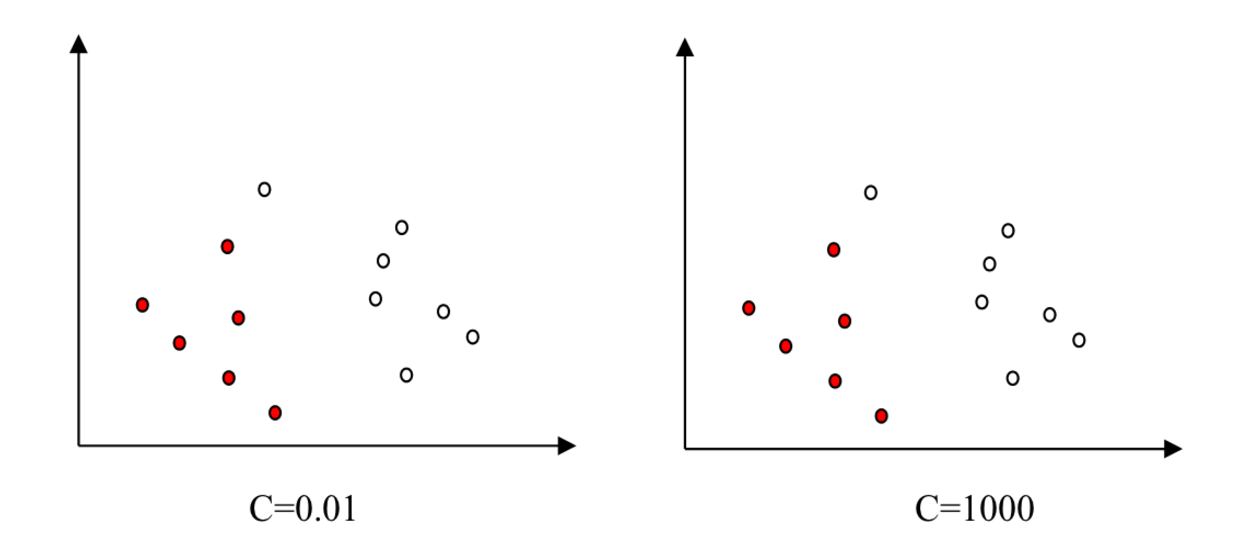
\includegraphics[width=6in]{2.eps}
    \pagebreak
	\item[3.] Consider applying SVM to the following two class classification problem. Please : \\
	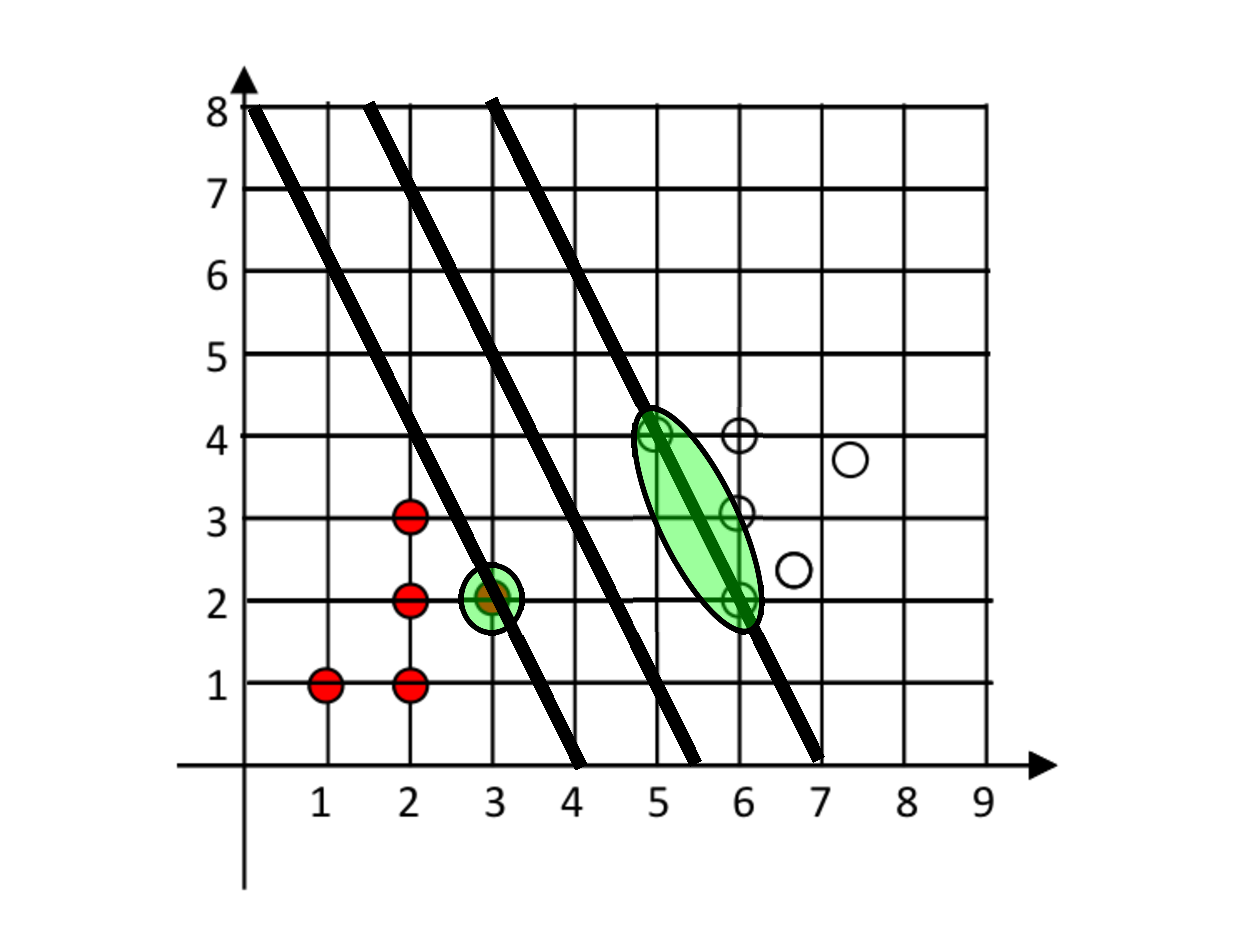
\includegraphics[width=4in]{3.eps}
	\begin{enumerate} 
		\item Mark out the fat decision boundary learned by SVM (this includes three lines $w\cdot x+b=0, w\cdot x+b=0, w\cdot x+b=1, w\cdot x+b=-1$). You should be able to identify the decision boundary by eyeballing, without actually solving the optimization problem. \\
		\item Circle the support vectors. \\
		\item What are the $w$ and $b$ parameter of this learned decision boundary (Hint: based on the support vectors, you hsould be able to plug their $x$ values in the correstponding equations and solve for $w$ and $b$). \\ \\
        point on $wx + b = 1$ is (3,2) \\
        point on $wx + b = 0$ is (5,1) \\
        point on $wx + b = -2$ is (6,2) \\
        $3*w_{1} + 2*w_{2} + b = -1$ \\
        $5*w_{1} + 1*w_{2} + b = 0$  \\
        $6*w_{1} + 2*w_{2} + b = 1$ \\
        Solving this system of equation yields the result \\
        $w_{1} = 2/3$ \\
        $w_{2} = 1/3$ \\
        $b = -11/3$ \\
	\end{enumerate}
	\item[4.] Create by hand the clustering dendrogram for the following samples of ten points in one dimension. Sample = $(-1.8, -1.7, -0.3, 0.1, 0.2, 0.4, 1.6, 1.7, 1.9, 2.0)$ 
	\begin{enumerate} 
		\item Using a single link. \\
		\item Using complete link. \\
	\end{enumerate} 
	Note that below are examples of dendrograms for the following three points $(1,2,4)$ with single and complete link. \\



\end{enumerate} 
\end{document} 
